%!TeX root = thesis-main.tex
%basicstyle=\fontsize{8}{9}\selectfont\ttfamily

%%%%%%% %%%%%%%%  %%%%%%% 
%%%%%%% COMMANDS  %%%%%%%
%%%%%%% %%%%%%%%  %%%%%%%


\sloppypar

%\chapter{Towards Reinforcement Learning-based Aggregate Computing}
\chapter{Program Sketching with Aggregate Computing}\label{chap:learning:sketching}
\minitoc% Creating an actual minitoc
\begin{comment}
The pervasiveness of computing and networking
 fosters applications 
 backed by large-scale cyber-physical collectives---cf. edge-fog-cloud infrastructures, robot swarms, %power grids, 
 and smart ecosystems.
%
Combined with the \emph{autonomic computing} vision ~\cite{DBLP:journals/computer/KephartC03}, which promotes autonomy and self-* capabilities in engineered systems,
 there is an increasing trend towards \acp{cas} and their engineering~\cite{DBLP:journals/sttt/NicolaJW20,DBLP:journals/tasm/BucchiaroneDPCS20}.
%
\acp{cas} are characterized 
 by a multitude of agents  
 that can produce globally coherent results (\emph{emergents}~\cite{DBLP:conf/atal/WolfH04}),
 and collective-level adaptivity to environment change
 via local decision-making and decentralized interaction.
%
The \emph{engineering of \acp{cas}} is an open research problem~\cite{DBLP:journals/sttt/NicolaJW20,DBLP:journals/corr/abs-1108-5643} of significance, tightly linked with the problems of ``steering'' self-organization and ``controlling'' emergence to promote desired while avoiding undesired emergents~\cite{DBLP:books/sp/08/Muller-SchloerS08}.
%
In general, when dealing with \acp{cas},
 there are two distinct problems:
 (i) given an initial system state and local behavioural rules, predicting what global outcomes will be produced (\emph{forward}, \emph{prediction}, or \emph{local-to-global problem});
 and
 (ii) what local behavioural rules must be assigned to the system devices to achieve certain global outcomes (\emph{inverse}, \emph{control}, or \emph{global-to-local problem}).
%
These two problems provide corresponding perspectives
 for \emph{designing} \acp{cas}.
% 
In particular, the latter perspective has promoted research on \emph{spatial} and \emph{macro-programming}~\cite{beal2013organizing-aggregate,DBLP:journals/corr/abs-2201-03473}
 aiming at expressing programs in terms of the desired global outcome
 and leaving the underlying platform to deal with the global-to-local mapping.

In this work,
 we consider \emph{\ac{ac}}~\cite{DBLP:journals/computer/BealPV15}, a prominent \emph{field-based coordination} approach~\cite{DBLP:journals/jlap/ViroliBDACP19} 
promoting macro-programming 
 by capturing \ac{cas} behaviours 
 as functions operating on \emph{computational fields}~\cite{DBLP:journals/jlap/ViroliBDACP19},
 in a system model of neighbour-interacting devices
 operating in asynchronous sense-compute-interact rounds.
%
A computational field is a macro-abstraction
 that maps a set of devices over time to computational values.
%
\ac{ac} is based on the \emph{\ac{fc}}~\cite{DBLP:journals/jlap/ViroliBDACP19}, or variants thereof,
 that define constructs for manipulating and evolving fields.
%
\end{comment}
\ac{cpsw} behaviour
 can be expressed by a single \emph{aggregate program} (global perspective)
 that also defines 
 what processing and communication activities
 must be performed by each individual device (local perspective).

Besides the programming model and its implications,
 a significant portion of research on \ac{ac}~\cite{DBLP:journals/jlap/ViroliBDACP19} has focussed
 on design and analysis of \emph{coordination algorithms} expressed in \ac{fc}
 for efficiently carrying out self-organising behaviours
 like, e.g., computing fields of minimum distances from sources (\emph{gradients})~\cite{DBLP:conf/ipsn/NagpalSB03,DBLP:journals/pervasive/MameiZL04,DBLP:conf/saso/AudritoCDV17},
 electing leaders~\cite{DBLP:conf/saso/MoBD18},
 or %collecting data %on spanning trees 
 %for 
 distributed summarization~\cite{DBLP:journals/cee/AudritoCDPV21}.
%
However, devising self-organising coordination algorithms is not easy; especially difficult is identifying solutions
 that are efficient across environment assumptions, configurations, and perturbations.
%
The difficulty lies in determining, 
 for a current context,
 the local decisions of each device, 
 in terms e.g. of processing steps and communication acts,
 producing output fields that quickly converge to the correct solution.

In chapter we adopt a \emph{\ac{rl}-based approach}---where an agent learns from experience
 how to behave in order to maximize delayed cumulative rewards~\cite{sutton2018reinforcement-learning}.
%
We devise a general methodology that somewhat resembles the notion of \emph{sketching} in program synthesis~\cite{solar2008program-synthesis-sketching}:
 a template program is given and \emph{holes} are filled with actions determined through search.
%
In our case, the program is the \ac{ac} specification of a coordination algorithm, and holes are filled with actions of a policy learnt through a multi-agent reinforcement learning algorithm called Hysteretic Q-Learning~\cite{DBLP:conf/iros/MatignonLF07}.
%
We consider the case of the classic gradient algorithm, a paradigmatic and key building block of self-organising coordination \cite{DBLP:journals/jlap/ViroliBDACP19,beal2013organizing-aggregate,DBLP:journals/corr/abs-2201-03473}: we show via simulations 
 that the system, after sufficient training,
 learns an improved way to compute and adjust gradient fields to network perturbations.

\section{On Integrating Machine Learning and Aggregate Computing}
As anticipated in \Cref{part:background}, 
 the behaviour of an aggregate system depends on the interplay of three main ingredients:
\begin{itemize}
  \item the aggregate program, expressing conceptually the global behaviour of the entire system, and concretely the local behaviour of each individual node in terms of local processing and data exchange with neighbours; and
  \item the aggregate execution model, promoting a certain dynamics of the system in terms of topology management (e.g., via neighbour discovery), execution of rounds, scheduling of communications; and
  \item  the environment dynamics.
\end{itemize}
%
While the latter cannot be controlled, 
 the importance of the first element is reflected by research
 on the design of novel algorithms (cf.~\cite{DBLP:journals/jlap/ViroliBDACP19,DBLP:conf/saso/AudritoCDV17}),
 while the second element is studied 
 w.r.t. the possibility of tuning and adaptivity 
 according to 
 available technology and infrastructure 
 or the dynamics of the environment---see the previous chapter. %(e.g. reacting to a phenomenon that changes quickly requires increasing the execution frequency---cf.~\cite{danilo2021lmcs}).
%
Since tuning programs or execution details to specific environments
 or adapting those to changing environments
 can be burdensome,
 it makes sense to consider the use of machine learning techniques
 to let a system \emph{learn} effective strategies for unfolding collective adaptive behaviour.
%

\section{Aggregate Programs Improvement through \ac{rl}}
%!TeX root = thesis-main.tex

\begin{figure}[t]
  \centering
  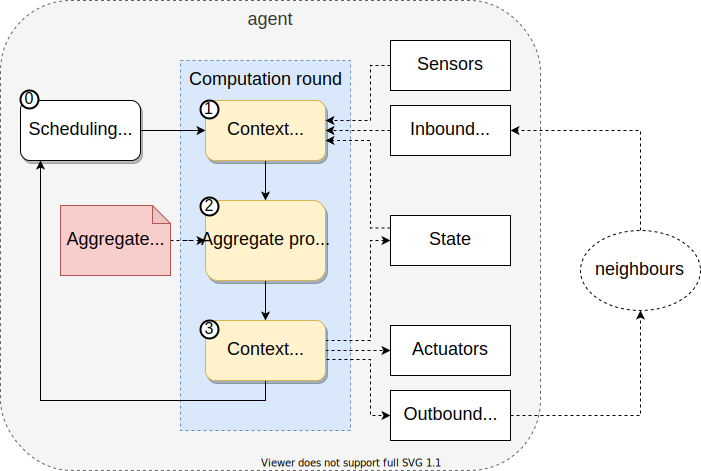
\includegraphics[width=0.9\textwidth]{papers/coordination2022/img/aggregate-agent-control-architecture.pdf}
  \caption[Integration of \ac{RL} within the \ac{ac} control architecture for collective program synthesis]{Integration of \ac{rl} within the \ac{ac} control architecture~\cite{DBLP:journals/jsan/CasadeiAV21}. 
  %
  The \ac{rl} state and reward concepts build upon the context, given by environment and neighbour data. 
  %
  The designer configures action points where learning can improve the aggregate computation. 
  %
  The actions selected by the learned policies will then affect the environment (via actuators) and neighbours (via outbound messages).}
  \label{coordination2022:fig:ac-and-rl}
\end{figure}

In this work, we focus on \emph{improving aggregate programs}
 by learning effective local actions
 within a given algorithmic schema---an approach similar to the \emph{sketching} technique for program synthesis~\cite{solar2008program-synthesis-sketching}.
Differently from the previous chapter, 
 where we used \ac{rl} to improve the execution model, 
 here we use \ac{rl} to improve the aggregate program.
% \meta{TODO: explain why RL and not other ML techniques}.
As a learning framework,
 we use \ac{rl} as 
 we deal with systems of agents 
 performing ongoing activities 
 by interacting with one another and the environment. 
 %it makes it possible to exploit learning even in cases where we do not know the optimal result for a certain program, but we can only evaluate its performance under certain circumstances (either with simulations or directly in concrete systems). 
% 
%From a local viewpoint, 
% an \ac{ac} device is an agent acting based on the local context it perceives (sensor readings, device state, and messages from neighbours), 
% and this matches the \ac{rl} execution model very well.

%So, our long-term goal is to integrate \ac{rl} into the \ac{ac} ``stack'' (i.e., across the platform, language, and library levels) to improve the collective behaviour defined by \scafi{} aggregate programs in terms of \emph{efficiency} (i.e., reducing the resource usage maintaining the same functional interface), \emph{efficacy} (i.e., synthesizing more stable and faster converging behaviours) and \emph{adaptability} (i.e., the same program works against different environments).
%

As a first contribution, summarized in \Cref{coordination2022:fig:ac-and-rl}, in this work we integrate \ac{rl} within the \ac{ac} control architecture in order to support learning of good collective behaviour sketched by a given aggregate program.
%
Specifically, 
 we focus on improving \ac{ac} building blocks (such as the gradient algorithm covered in \Cref{coordination2022:sec:gradient}) through learning, leading toward a so-called \emph{Reinforcement Learning-based Aggregate Computing}. 
%
Learning, thus, does not replace the \ac{ac} methodology for defining the programs, 
 but it is best understood as a technique that supports and improves the \ac{ac} algorithm design process. 
\section{Building blocks Refinement}\label{coordination2022:s:learning-gradient}
A major advantage of \ac{ac} as a programming model is its \emph{compositionality}: complex collective behaviours (e.g., the maintenance of a multi-hop connectivity channel) can be expressed through a combination of building blocks capturing simpler collective behaviours (e.g., gradients).
%
Since building blocks are fundamental bricks of behaviour that often recur in programs, 
 their bad and good qualities (cf., convergence speed, stability, etc.) tend to amplify and affect behaviours that depend on them.
%
%Even if AC is independent of IT infrastructure, several behaviours tend to have a long self-stabilisation time in some deployments w.r.t the idealised convergence time, leading to non-stable and unpredictable aggregate programs.
%
Therefore, research tends to investigate refined variants of building blocks that provide the same functionality but are more \emph{effective} or \emph{efficient} under specific assumptions or contexts (e.g., high mobility, situations where stability is more important than precision, etc.)~\cite{DBLP:conf/saso/AudritoCDV17,DBLP:journals/cee/AudritoCDPV21}.
%
With a library of algorithms, 
 the designer can choose the best combination of building blocks that are well-fitted for a given environment, 
 and even substitute a building block with a variant implementation without substantially affecting the application logic.
%\meta{@GA to @All, in sec 4.1 I show a gradient block with opt. Probably here we need to show a general structure? With images? }
In general, a building block can be seen as a \emph{black box} (function) that takes a set of input fields (e.g. metric, perception fields, constant fields, etc.) and yields an output field. 
%
To increase its flexibility, 
 such a function could leverage a \emph{refinement policy} able to affect the behaviour of the building block over time or in a certain situation. 
%
This policy could be a feedback loop, hysteresis, or custom logic to solve a specific problem.
%
We aim at structuring the learning of refinement policies through \ac{rl}~\cite{DBLP:conf/acsos/Aguzzi21}.
%
Our idea is that it should not be the designer who codes a particular block to be used, 
 but that it is the learning algorithm that understands, given a global policy to be optimized following a utility function, 
 what actions need to be activated.
% to optimise the collective good of the system.

%!TeX root = paper22-coord-ac-rl.tex
\begin{figure}[t]
  \includegraphics[width=\textwidth]{papers/coordination2022/img/algorithm-learning.pdf}
  \caption[Reinforcement Learning schema used in program synthesis simulations]{
  Reinforcement Learning schema used in our simulations.
  The learning algorithm is applied at simulation time (for $T$ episodes) improving a shared $Q$ table. 
  %
  At the deployment time then, the agents exploit a local copy of the optimal $Q^*$ table found by learning.}
  \label{coordination2022:fig:learning-scheme}
\end{figure}

The continuous and variable state problems are typically tackled using Deep Learning to learn the right state representation for a given problem~\cite{DBLP:journals/corr/abs-1806-08894}. %and Graph Neural Networks (to regulate variable-size inputs). 
%
In this case, instead, we used a handcraft feature engineering process since we are more interested in devising a general design process.

Concerning the \emph{multi-agent credit assignment problem}, we decided to use offline learning 
%based on simulation and then the policy is deployed in a concrete system 
in a typical \ac{ctde} setting (\Cref{coordination2022:fig:learning-scheme}).
%
This way, we assess the influence of an individual in comparison to the entire system, which cannot be done in online learning due to the difficulty of achieving global snapshots of the system in a reasonable time.


\section{Learning Schema} 

The learning algorithm is seen as a state ($s_t$) evolution function in which the nodes try to apply a correction factor (\lstinline|update|) following a policy ($\pi^Q_{target}$ or $\pi^Q_{behavioral}$) refined by learning.
%
The state is built from a neighbourhood field of the building block generic output ($o_t$) passed as input.
%
\Cref{coordination2022:lst:general-schema} exemplifies the general program structure used to combine \ac{rl} with \ac{ac} for improving building blocks.
%
The branching operator (\lstinline|branch|) on \lstinline|learn| condition makes it possible to use the \ac{ctde} schema since when the \lstinline|learn| is \lstinline|false| there is no need for a central entity (\lstinline|simulation|).
%
The Q table is gathered using \lstinline|sense|, a \scafi{} operator used to query sensors and collect data from them. 
%
At simulation time, Q is a shared object, but at runtime each agent owns a local table.
%
%!TeX root = paper22-coord-ac-rl.tex

\begin{lstlisting}[
  mathescape,
  %float=tp,
  floatplacement=tbp,
  frame=single,
  label={lst:general-schema},
  caption={
    ScaFi-like pseudocode description (implemented in the simulation) for value-based \ac{rl} algorithm applied \ac{ac}.
    %
    \texttt{state}, \texttt{update}, \texttt{reward} are block specific. 
    %The learn branch use \texttt{simulation}, a global object in which agents access to a shared Q.
  },
  captionpos=b
]
def optBlock($o_{t-1}$) { // learning as a field that evolves in time
  rep(($s_0, a_0$, $o_0$)) { // $s_0$, $a_0$ context dependent 
    case ($s_{t-1}, a_{t-1}$, _) => {
      val Q = sense("Q") // global during training, local during execution
      val $o_{t}$ = update($o_{t-1}$, $a_{t-1}$) // local action
      // state from the neighbourhood field program output
      val $s_{t}$ = state(nbr($o_{t}$))
      val $a_{t}$ = branch(learn) { // actions depends on learn condition
        val $r_{t-1}$ = reward($o_{t}$, simulation) // simulation is a global object
        simulation.updateQ(Q, $s_{t-1}$, $a_{t-1}$, $r_{t-1}$, $s_{t}$) // Q update
        $\sim$ $\pi_{behavioural}^Q$($s_{t}$) // sample from a probabilistic distribution
      } {
        $\pi_{target}^Q$($s_t$) // greedy policy, no sampling is needed
      }
    }
    ($s_{t}$, $a_{t}$, $o_{t}$) 
  }._3 // select the output from the tuple
}
  \end{lstlisting}
  %\caption{\scafi{}-like pseudocode description for value-based \ac{rl} algorithm applied \ac{ac}. \texttt{state}, \texttt{update}, \texttt{reward} are block specific. The learn branch use \texttt{simulation}, a global object in which agents access to a shared Q. 
  %$\sim$ stands for sampling a value from a probabilistic distribution.}
  %\label{lst:general-schema}
%\end{figure}
%
Finally, the produced $o_{t}$ is returned to the caller.

In this case, we encoded the learning process with \ac{ac} itself. 
%
Though we could have extracted the learning process from the \ac{ac} program, %producing a policy usable in \ac{ac},
 we took this decision because: 
  (i) it allows us to extend learning by exploiting neighbourhood Q table fields -- so we can think of doing non-homogeneous learning in different areas of the system;
  (ii) the scheme for taking state and choosing actions is the same as the one we would need for learning, so the only difference is in the branch; and
  (iii) it can simply be extended to online learning.
%
%In the next section, we describe an incarnation of this algorithm applied to the gradient block.

\section{Reinforcement Learning-based gradient block}
%\meta{
%  \begin{itemize}
%    \item describe the block G -- why it is important, for what is used 
%    \item G problems -- stable results, count-to-infinity, speed bias
%    \item try to describe a general G block that accept an optimisation/correction strategy
%    \item define the Reinforcement Learning as an optimisation block
%  \end{itemize}
%}

%\meta{@GA to @All: another way to generalise G?}
The gradient block could be generalized as follows:
\begin{lstlisting}
def gradientOpt(source, metric, opt) {
  rep(infinity) { g => mux(source) { 0 } { opt(g, metric) } }
}
\end{lstlisting}
where \lstinline|opt| is a function that determines how to evolve the gradient based on the field of current gradient values \lstinline|g| and current \lstinline|metric| (estimation of distances to neighbour). 
%In this way, the correction factor applied to the gradient could be composed, creating a gradient block that handles several scenarios.
In this article, we consider \lstinline|opt| as a \emph{hole} that a \ac{rl} algorithm will fill through raw experience
 with actions aiming at incrementally constructing a gradient field, hopefully mitigating the \emph{rising-value} issue (cf. \Cref{coordination2022:sec:gradient}).
%
To frame our learning problem, we adopt the above-described general schema (\Cref{coordination2022:fig:learning-scheme}). The state and action functions are inspired by the CRF algorithm.
%
The \lstinline|state| function must hold enough information to know when agents should speed up the local rising of values.
%
In this case, we encode the state as the difference between the output perceived by a node and the minimum and maximum gradient received by its neighbours: $s_t = (|min_t - o_t|, |max_t - o_t|)$. 
%
These data have to be discretized; otherwise, the search space would be too big and the solution could suffer from overfitting. 
%
The discretization is ruled by two variables, $maxBound$ and $buckets$. 
%
The former constrains the output to be between $ - radius * maxBound$ and $ radius * maxBound $ (where $radius$ is the maximum communication range of the nodes). 
%
The values outside that range will be considered as the same state.
%
The $buckets$ variable rules the division count of the given range. 
Finally, we stack two time steps in order to encode history inside the agent state:
$h_t = [(s_{t - 1}, s_t)]$. $h_t$ is used as the state function for our \ac{rl} algorithm.
Hence, the cardinality of the state space of $|s_t| * |s_t| = buckets^4$. 
%
The action space is divided into two action types: \texttt{ConsiderNeighbourhood} is the action that will produce the classic gradient evaluation, while 
 \texttt{Ignore(velocity)} ignores the neighbour data and increases the gradient at a given \texttt{velocity}. So, the \texttt{update} function is defined as:
\begin{lstlisting}[mathescape]
def update($o_{t-1}$, $a_{t-1}$, metric) = // $o_{t-1}$ is the previous gradient output
  val $g_{classic}$ = minHoodPlus(nbr($o_{t-1}$) + metric())
  match $a_{t-1}$ // scala-like pattern matching
    case ConsiderNeighbourhood => $g_{classic}$
    case Ignore(velocity) => $o_t$ + velocity * deltaTime() 
\end{lstlisting}
%
Finally, the \texttt{reward} function is described as follows: 
\begin{lstlisting}[mathescape]
def reward($o_t$, simulation) {
  if($o_t$ - simulation.rightValueFor(mid()) $\sim$= 0) { 0 } { -1 }
}
\end{lstlisting}
where \lstinline|mid| returns the field of node identifiers. 
%%
The idea is to push the nodes to produce an output that is very close to the ideal, correct gradient value as provided by an oracle (\lstinline|simulation.rightValuefor()|).
%%
When this is the case, we provide a value equals to $0$;
instead, when the value is different from the expected one, 
 we provide a small negative reward, $-1$, in order to push the nodes to quickly seek the situation where the actual and ideal value match.

\section{Evaluation}\label{coordination2022:s:eval}

\begin{table}[t]
  \centering
  \begin{tabular}{|c|c|}
    \hline
    Name &  Values \\ \hline
    $(\gamma)$ & [0.4 -- 0.7 -- 0.9] \\  \hline
    $(\epsilon_0, \theta)$ & [(0.5,200) -- (0.01,1000) -- (0.05,400) -- (0.02,500)] \\ \hline
    $(\beta, \alpha)$ & [(0.5,0.01) -- (0.5,0.1) -- (0.3,0.05) -- (0.2,0.03) -- (0.1,0.01)]
    \\  \hline
    (buckets, maxBound) & [(16,4) -- (32,4) -- (64,4)]\\ \hline
  \end{tabular}
  \caption{Summary of the simulation variables. 
  %
  A simulation is identified by a quadruple $(i, j, k, l)$ of indexes for each variable. 
  %
  %So simulation 0000 is the one with $\gamma = 0.4, \epsilon_0 = 0.5, \theta = 200, \beta = 0.5, \alpha = 0.01, buckets = 16,  maxBound = 4$.
  }
  \label{coordination2022:table:parameters}
\end{table}

To evaluate our approach, we run a set of simulated experiments and verify that an aggregate system
 can successfully learn an improved way to compute a gradient field (cf. the gradient block described in \Cref{coordination2022:sec:gradient}).
%
To this purpose, we adopt Alchemist~\cite{DBLP:journals/jos/PianiniMV13},
 a flexible simulator 
 for pervasive and networked systems
 that comes with a support for aggregate systems 
 programmed with \scafi{}~\cite{DBLP:conf/isola/CasadeiVAD20}. 
%
The source code, data, and instructions for running the experiments have been made fully available at a public repository\footnote{\url{https://github.com/cric96/experiment-2022-coordination}}, to promote reproducibility of results.

\subsection{Simulation setup}

The simulated system consists of $N$ devices deployed in a grid. 
%
We use two kinds of grid-like environments. 
%
They both have the same width (\SI{200}{\metre}) and distance between nodes (\SI{5}{\metre}), but they differ in the row count. 
%
In one case, only one row exists (so the nodes are placed in a line). 
%
In the other case, there are five rows. 
%
The total number ($N$) of agents is then defined as $ 200 / 5 * rows $. 
%
So in the first case, we have a total of 40 agents, in the second case we have 200 agents. 
%
Each node asynchronously fires the round evaluation at \SI{1}{\hertz}.
%
The leftmost and the rightmost agents are marked as source nodes. 
%
Each simulated episode lasts \SI{85}{\second} ($T$).
%
For simulating the slow rising problem, we drop the left source at \SI{35}{\second} ($C_s$), and so the left part of the system starts to rise until eventually stabilizing to the correct computational field.
%
An entire simulation lasts $N_E = 1200$ episodes, in which in the first $N_L = 1000$ the system uses \ac{rl} to improve a shared Q table, and then in the last $N_T = 200$, the system deploys the Q table found in each agent. 
%
In these last runs, the agents act following the greedy policy.

As learning algorithm, we used Hysteretic Q-Learning (cf. \Cref{coordination2022:s:background:rl}). %, since it tackles environments stochasticity.
%
As behavioural policy, we use an $\epsilon$-greedy with an exponential decay to balance the exploration-exploitation.
%
We make this choice because without using the decay the policy found tends to be not optimized (i.e. the exploration is preferred w.r.t exploitation).
%
At each episode $i$, the $\epsilon$ value is updated as $\epsilon_i = \epsilon_0 \cdot e^{{i} / \theta}$.

Several variables are used, summarized in \Cref{coordination2022:table:parameters}, so we perform a grid search to find the optimal combination.
%
To evaluate a particular configuration, we verified the total error performed in the last $N_T$ episodes.
%
This is calculated from the error performed by each node $i$ at each time step $t$:
\begin{equation}
error_i^{t} = |gradient_i^{t} - simulated_i^t|
\end{equation}
Then for each time step $t$, we evaluate the average system error as:
\begin{equation}
error_{t} = \frac{1}{n}\sum_{i = 0}^N error_i^t
\end{equation}
And finally, the error of each episode is evaluated as:
\begin{equation}
error_{episode} = \sum_{t = 0}^T error_{t}
\end{equation}
We choose the configuration by observing the box plots (\Cref{coordination2022:subfig:boxplot}) and taking the lowest average error in the last $N_T$ episodes.

%!TeX root = paper22-coord-ac-rl.tex
\newcommand{\figfactor}{0.45}
\begin{figure}[t!]
  \bigskip
  \begin{subfigure}[t]{\figfactor\textwidth}
    \centering
    \includegraphics[width=\textwidth]{papers/coordination2022/img/box-all.pdf}
    \caption{Box plots of last $G_s$ episode.}
    \label{subfig:boxplot}
  \end{subfigure}  
  \hfill
  \begin{subfigure}[t]{\figfactor\textwidth}
    \centering
    \includegraphics[width=\textwidth]{papers/coordination2022/img/mean-error-left.pdf}
    \caption{Learning progress of the best result.}
    \label{subfig:mean-error-over-episode}
  \end{subfigure}
  \bigskip
  
  \begin{subfigure}[t]{\figfactor\textwidth}
    \centering
    \includegraphics[width=\textwidth]{papers/coordination2022/img/error-few-nodes.pdf}
    \caption{Error evolution with 40 agents}
    \label{subfig:error-few}
  \end{subfigure}
  \hfill
  \begin{subfigure}[t]{\figfactor\textwidth}
    \centering
    \includegraphics[width=\textwidth]{papers/coordination2022/img/error-many-nodes.pdf}
    \caption{Error evolution with 200 agents}
    \label{subfig:error-many}
  \end{subfigure}
  \bigskip
  
  \begin{subfigure}[t]{\figfactor\textwidth}
    \centering
    \includegraphics[width=\textwidth]{papers/coordination2022/img/output-few-nodes.pdf}
    \caption{Output evolution with 40 agents}
    \label{subfig:output-few}
  \end{subfigure}
  \hfill
  \begin{subfigure}[t]{\figfactor\textwidth}
    \centering
    \includegraphics[width=\textwidth]{papers/coordination2022/img/output-many-nodes.pdf}
    \caption{Output evolution with 200 agents}
    \label{subfig:output-many}
  \end{subfigure}
  \caption{Performance of our \ac{rl}-based gradient algorithm with \lstinline|velocity| = 20.
  }
  \label{fig:eval}
\end{figure}
\subsection{Results and Discussion}

\Cref{coordination2022:fig:eval} shows the performance of our \acl{rl}-based gradient algorithm.
%
\Cref{coordination2022:subfig:boxplot} was used to choose which configuration was the best.
%
\Cref{coordination2022:subfig:mean-error-over-episode} shows the error trend as the episodes change. 
%
The second row shows the trend of the mean error over the last $N_T$ episodes. 
%
The coloured area under the curve defines the standard deviation. 
%
The dashed vertical line is the time at which the source change occurs. 
%
Finally, the last row shows the average output of the various algorithms. 
%
In the following we discuss the result reached with the best configuration, that has $\gamma = 0.9$, $\epsilon_0 = 0.5$, $\theta = 200)$, $\alpha=0.3$ and $\beta=0.05$. 

Our goal was to create a solution that outperforms the classic gradient against the rising-value problem.
%
In fact, the system eventually learns how to speed up the gradient rising: observing the \Cref{coordination2022:subfig:mean-error-over-episode} the $error_{episode}$ of the new algorithm is lower than the error produced by the standard solution. 
%
In particular, this means that the agents learn the moment when they should ignore their neighbourhood and increase the output with a certain velocity (i.e. using the \lstinline|Ignore| action).

This intuition is enforced by \Cref{coordination2022:subfig:error-few,coordination2022:subfig:error-many,coordination2022:subfig:output-few,coordination2022:subfig:output-many}.
% 
In particular, in \Cref{coordination2022:subfig:error-few,coordination2022:subfig:output-few} the behaviour is more evident due to the reduced number of agents: when the error is maximized (due to the source that disappears), the error decreased faster than the naive gradient (and, consequently, the output is faster growing).
%
Furthermore, we can also observe that the overall algorithm behaviour is comparable with the CRF handcrafted solution for the rising problem. 
%
Indeed, both have a phase of speed up followed by another phase of overestimation (i.e. the system-wide output is greater than the true gradient field output) that eventually brings the system to slowly reaches the correct value.
%
Moreover, not only the \ac{rl}-based solution has similar behaviour to CRF, but also it has comparable performance -- it means that the aggregate reaches a near-optimal policy with these state-action-reward settings.

We want also to underline that the policy learned is \emph{one} and shared with the whole system.  
%
Thereby, the policy can be easily scaled in deployments with different node counts. 
%
In this case, the \emph{same} function outperforms our baseline in a system with different nodes and deployment configurations. 
%
%The current issue is, however, that we cannot prove that this policy works with any possible deployment: this needs to be evaluated in future work.

Finally, we want to stress that the nodes do not fire synchronously, and thus there is not any kind of global and shared clock: any node round evaluation order reaches the same behaviour in our test deployments. 
%
This, again, makes it possible to use the same policy in different scenarios due to the unknown local aggregate programs evaluation order.

\section{Wrap up}\label{coordination2022:s:conc}

This chapter discusses the integration of \acl{ac} -- a programming approach for \aclp{cas} -- and \acl{rl}, with the goal of fostering the design of collective adaptive behaviour.
% 
In particular, we propose to use \ac{rl} as a means to improve building block \ac{ac} algorithms. %- in a similar way to what is done in program synthesis. 
%
Our approach is applied to improving the gradient algorithm, one of the key \ac{ac} algorithms, where learning is performed through Hysteretic Q-Learning.
%
We evaluate the approach through synthetic experiments comparing the reactivity of different gradient algorithms in dealing with the rising value problem.

%\printbibliography